%%%%%%%%%%%%%%%%%%%%%%%%%%%%%%%%%%%%%%%%%
% Bible (Three-Column)
% LaTeX Template
% Version 1.0 (06/29/26)
%
% Original author:
% PSALMS to God (www.psalmstogod.com)
% 
%
%%%%%%%%%%%%%%%%%%%%%%%%%%%%%%%%%%%%%%%%%

%----------------------------------------------------------------------------------------
%	PACKAGES AND DOCUMENT CONFIGURATIONS
%----------------------------------------------------------------------------------------

% AI Prompt: watercolor style title page for the book of Daniel including author (Daniel), Hebrew name of the book ( דניאל) and the fact that it is part of the Major Prophets and Ketuvim ( כתובים). Center image should reference the contents of this book and if any people are depicted they should be of various skin tones. 

% Alt AI Prompt: studio ghibli inspired cover page for the book of Ruth. It should include the Hebrew name (רוּת), author (Joshua), date of authorship (1010–970 BCE), the Jewish and Christian classifications of the book (נְבִיאִים and Books of History, respectively), and images representing the themes of the book. People should have varying skin colors. Imagery should be based on the plot and themes of the book (battles, division of the land, fall of Jericho, Rahab, etc.)

\documentclass[8pt,letter,twoside,openany]{extbook}


\usepackage{tabularx} %tables
\usepackage{multicol} %for two columns
\usepackage[toc]{multitoc} %two column table of contents
\usepackage[table]{xcolor}
\usepackage{lettrine}		%for drop numbers
\usepackage{fancyhdr}
\usepackage{titlesec}		%for drop numbers & headers
\usepackage[Rejne]{fncychap}  % chapter style
\usepackage{xparse}	    	%for drop numbers
\usepackage{geometry}	%for margins
\usepackage[symbol,perpage]{footmisc}	%footnotes as symbols

\usepackage{fontspec}	% allows specification of font (for Hebrew)
\usepackage{changepage} %for quotes/spacing/indenting
\usepackage{graphicx} %for inserting images
\usepackage{hyperref} %links
\usepackage{pdfpages} % for full page images
% Load babel with English and Hebrew support, enabling bidirectional layout
\usepackage[english, bidi=basic]{babel}

% Import the Hebrew language configuration
\babelprovide[import]{hebrew}
\babelfont{rm}{Arial} % Replace with any font on your system that supports Hebrew

\definecolor{crimson}{HTML}{B22222}


\DeclareRobustCommand{\mybook}[1]{% <-- Safe, robust global macro structure
	\chapter*{#1}% Prints the unnumbered main chapter title
	\gdef\currentchaptername{#1}% Safely sets the string globally
	\markboth{#1}{#1}% Safely sets the native header title globally
	\setcounter{section}{0}% Resets section numbers
	\InsertMark{autonumbers}{0:0}% Resets verse registers for page bounds
}
%set up mark sytem for headers
\NewMarkClass{autonumbers}

% Define drop numbers for chapters within a book
\renewcommand{\thesection}{\arabic{section}}


\titleformat{\section}
{\normalfont\fontseries{b}\selectfont\filright} % Font styling
{}{0pt}{} % No raw default label prefix
\titlespacing{\section}
{0pt}{.2ex plus .1ex minus .2ex}{1pc} % Margin formatting adjustments


\NewDocumentCommand{\mychapter}{ O{#2} m }{%
	\section[#1]{#2}%
	% Baseline mark for headers if a page breaks exactly at a title
	\InsertMark{autonumbers}{\thesection:1}% 
	\setcounter{myversecount}{0}%
	% Trigger the lettrine drop cap instantly and safely on the text following the title
	\lettrine[lines=2,nindent=0pt,findent=2pt]{\textbf{\thesection}}{}%
}


% Define superscript verse numbers
\newcounter{myversecount}[section]
\renewcommand{\themyversecount}{\arabic{myversecount}}

\NewDocumentCommand{\myverse}{s}{%
	\refstepcounter{myversecount}%
	%\markboth{\thesection:\arabic{verse}}{}%
	\InsertMark{autonumbers}{\thesection:\arabic{myversecount}}
	\IfBooleanF{#1}{\textsuperscript{\arabic{myversecount}}}%
}
%------------------------------------------------

% Define margins
\geometry{
	inner=20mm,  % Margin closest to the binding
	outer=60mm,  % Margin on the outside edge (allows for journaling space)
	top=17mm,
	bottom=14mm
}
%------------------------------------------------
% Set Headers for pages
\pagestyle{fancy}
\fancyhf{}
\fancyhead[OL]{\thepage}
\fancyhead[OR]{\currentchaptername \hspace{.5mm} \FirstMark{autonumbers} --- \currentchaptername \hspace{.5mm}\LastMark{autonumbers}}
\fancyhead[ER]{\thepage}
\fancyhead[EL]{\currentchaptername \hspace{.5mm} \FirstMark{autonumbers} --- \currentchaptername \hspace{.5mm} \LastMark{autonumbers}}

%------------------------------------------------

\setcounter{tocdepth}{0}	% for the table of contents depth ( only show chapter)

%  FIX: Manual definitions to bypass the titlesec + extbook bug
\renewcommand{\frontmatter}{%
	\clearpage
	\pagenumbering{roman}% Lowercase roman numerals for intro pages
	\pagestyle{empty}% Turns headers OFF for the intro section globally
}

\renewcommand{\mainmatter}{%
	\clearpage
	\pagenumbering{arabic}% Swaps page tracking back to 1, 2, 3...
	\setcounter{page}{1}% Explicitly restarts the tracking page count at 1
	\pagestyle{fancy}% Turns your custom range headers ON safely
}

\begin{document}
\frontmatter
\input{frontmatter.tex}

\mainmatter
% OLD TESTAMENT
\addcontentsline{toc}{part}{OLD TESTAMENT}
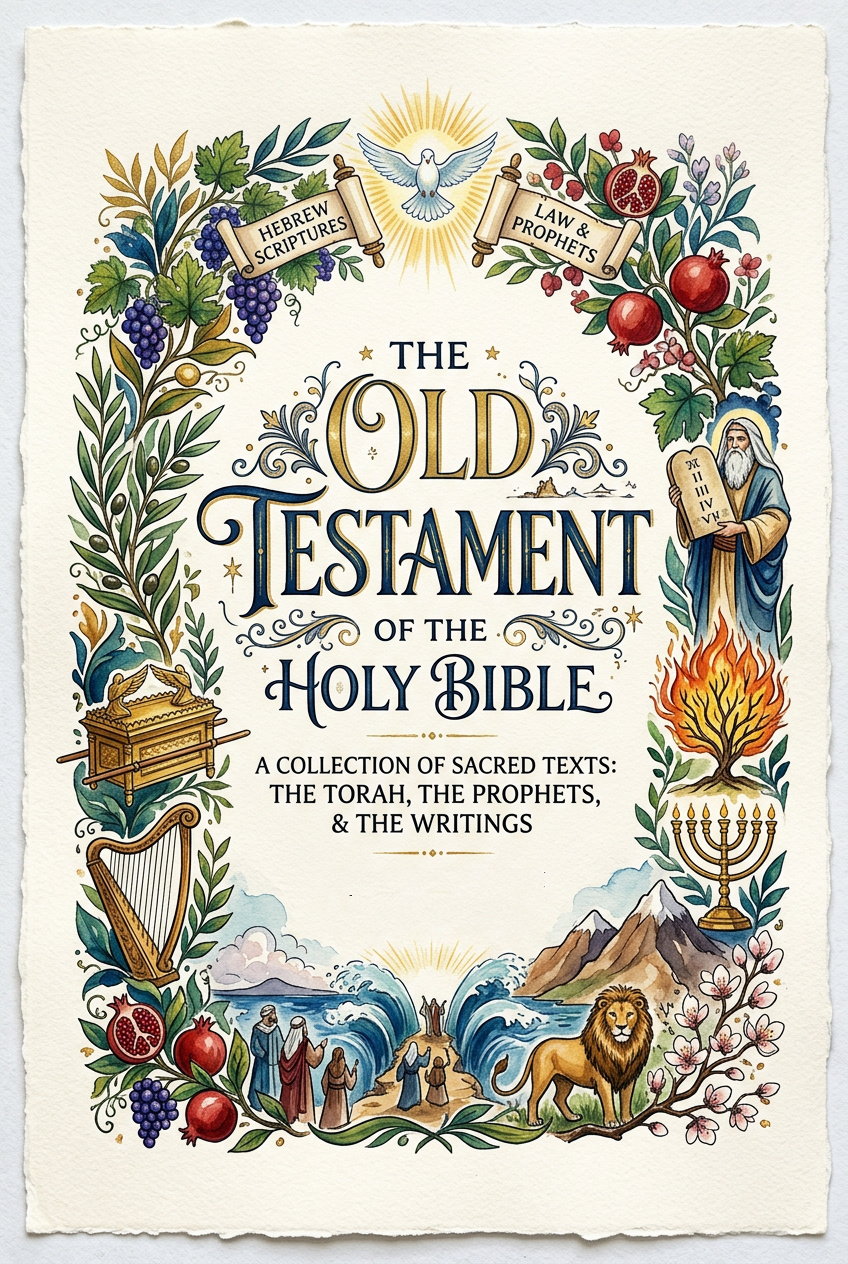
\includepdf[pages=1, fitpaper=false, width=\paperwidth, height=\paperheight, , keepaspectratio=false]{images/oldtestament.png}

\newpage
\null
\thispagestyle{empty}
\newpage

% Hebrew order
	\include{genesis.tex} 
	\include{exodus.tex} 
	\include{leviticus.tex}
	\include{numbers.tex}
	\include{deuteronomy.tex}
	
	\include{joshua.tex}
	\include{judges.tex}
	\include{1_samuel.tex}
	\include{2_samuel.tex}
	\include{1_kings.tex}
	\include{2_kings.tex}
	\include{isaiah.tex}
	\include{jeremiah.tex}
	\include{ezekiel.tex}

\include{hosea.tex}
\include{joel.tex}
\include{amos.tex}
\include{obadiah.tex} 
\include{jonah.tex}
\include{micah.tex}
\include{nahum.tex}
\include{habakkuk.tex}
\include{zephaniah.tex}
\include{haggai.tex}
\include{zechariah.tex}
\include{malachi.tex}


\include{psalms.tex}
\include{proverbs.tex}
\include{job.tex}
\include{song-of-solomon.tex}
\include{lamentations.tex}
\include{ecclesiastes.tex}
\include{esther.tex}
\include{ruth.tex}
\include{daniel.tex}
\include{ezra.tex}
\include{nehemiah.tex}
\include{1_chronicles.tex}
\include{2_chronicles.tex}

\newpage
\null
\thispagestyle{empty}
\newpage
\addcontentsline{toc}{part}{NEW TESTAMENT}
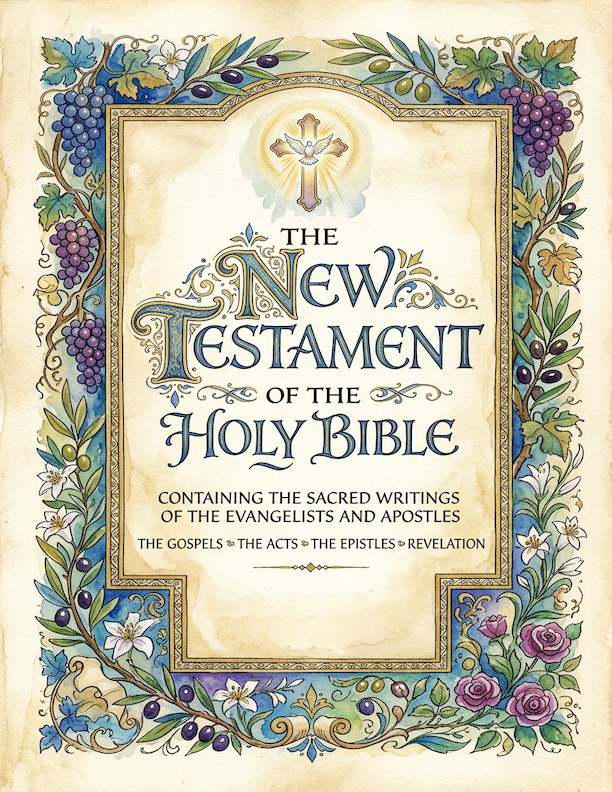
\includepdf[pages=1, fitpaper=false, width=\paperwidth, height=\paperheight, , keepaspectratio=false]{images/newtestament.png}
\newpage
\null
\thispagestyle{empty}
\newpage
	
% NEW TESTAMENT
	\include{matthew.tex}
\include{mark.tex}
\include{luke.tex}
\include{john.tex}
\include{acts.tex}
\include{romans.tex}
\include{1corinthians.tex}
\include{2corinthians.tex}
\include{galatians.tex}
\include{ephesians.tex} 
\include{philippians.tex}
\include{colossians.tex}
\include{1thessalonians.tex}
\include{2thessalonians.tex}
\include{1timothy.tex}
\include{2timothy.tex}
\include{titus.tex}
\include{philemon.tex}
\include{hebrews.tex} 
\include{james.tex}
\include{1peter.tex}
\include{2peter.tex}

\begingroup
\renewcommand{\clearpage}{}
\renewcommand{\cleardoublepage}{}
\include {1_john.tex}
\include{2_john.tex}
\include{3_john.tex}
\endgroup

\include{jude.tex}
\include{revelation.text}% TODO
	
\end{document}